\documentclass[11pt,letterpaper]{exam}
%\usepackage[Lhdr={},Rhdr={}]{plain}

\newtheorem{proposition}{Proposition}
\newcommand{\blue}[1]{\textcolor{blue}{#1}}
\newcommand{\red}[1]{\textcolor{red}{#1}}
\newcommand{\white}[1]{\textcolor{white}{#1}}

\usepackage{tikz}
\usetikzlibrary{shapes.geometric}
\usepackage{pgfplots}
\usetikzlibrary{patterns, pgfplots.fillbetween}
\usepackage{graphicx}
\usepackage{verbatim}
\usepackage{subfigure}
\usetikzlibrary{positioning}
\usetikzlibrary{snakes}
\usetikzlibrary{calc}
\usetikzlibrary{arrows}
\usetikzlibrary{decorations.markings}
\usetikzlibrary{shapes.misc}
\usetikzlibrary{matrix,shapes,arrows,fit,tikzmark}
\usepackage{amsmath}
\usepackage{mathpazo}
\usepackage{hyperref}
\usepackage{lipsum}
\usepackage{multimedia}
\usepackage{graphicx}
\usepackage{multirow}
\usepackage{graphicx}
\usepackage{dcolumn}
\usepackage{bbm}
\usepackage{comment}
 \usepackage{booktabs}
\usepackage{tabularx}
\usepackage{adjustbox}
\usepackage{graphicx}
\usepackage{multicol}
\usepackage{mathtools}
\usepackage[table,xcdraw]{xcolor}
\usepackage[top=0.5in,
  headsep=0pt% remove space between header and text body
  ]{geometry}
\usepackage{lastpage}
\cfoot{Page \thepage \hspace{1pt} of \pageref{LastPage}}

\newcommand{\figpath}{figs/}

\usepackage{titlesec}
\titleformat*{\section}{\large\bfseries}

\begin{document}


\begin{center}

{\large

\textbf{Problem Set 1}

}
\end{center}

\begin{questions}

\question  Consider the Two-Country, Two-Goods Ricardian model that we have studied in class. There are two countries $i \in \{ US,COL \}$ and two products $p \in \{R,C \}$.

\begin{parts}
\part  In each country, there is a representative household with preferences over the consumption of each good $Q_{i,p}$ denoted by an utility function $U_{i}(Q_{i,R} , Q_{i,C})$, taking goods prices $P_{i,p}$ as given. They supply labor $L_i$ inelastically for wage $w_i$. Suppose that consumer preferences are Cobb-Douglas with weight $0 < \alpha_i < 1$. Write down the consumer utility maximization problem, including the budget constraint.

\textcolor{red}{\begin{align*}
\max_{\{Q_{i,R},Q_{i,C}\}} Q_{i,C}^{\alpha_i}Q_{i,R}^{1-\alpha_i} \qquad s.t. \qquad P_{i,R}Q_{i,R} + P_{i,C}Q_{i,C} = w_i L_i
\end{align*}}

\part Provide an economic interpretation for how the utility function represents preferences. (hint: think of how utility changes as consumption changes).

\textcolor{red}{(a) Utility increases as consumption of either team increases ($\partial U_{i} / \partial Q_{i,p} >0$). (b) As consumption of one good increases for a fixed consumption of the other good, it does so in an decreasing rate. In other words, the utility function exhibits diminishing marginal returns ($\partial^2 U_{i} / \partial Q_{i,p}^2 <0$).  }


\part Provide and economic interpretation for the Cobb Douglas weight $\alpha_i$.


\textcolor{red}{The weight $\alpha_i$ controls how much the consumer prefers (subjectively) one good relative to the other. If $\alpha_i\to1$, consumer values $Q_{i,C}$ much more (for fixed prices). Conversely, if $\alpha_i\to0$, consumer values $Q_{i,R}$ much more (for fixed prices).}

\part Provide an economic interpretation for the budget constraint. What does each side of the equation represents?

\textcolor{red}{ TOTAL EXPENDITURE = TOTAL INCOME}

\part Chart the indifference curves as a function of demand choices $Q_{i,R},Q_{i,C}$. Explain what these curves mean.

\part Using the budget constraint, replace for $Q_{i,R}$ in the objective function and derive an expression for $Q_{i,R}$ as a function of $Q_{i,C}$ (or vice versa).
\textcolor{red}{
(i) re-state maximization problem
\begin{align*}
    Q_{i,R} &= \frac{w_i L_i}{P_{i,R}} - \frac{P_{i,C}}{P_{i,R} } Q_{i,C} \\    
    \max_{\{Q_{i,C} \}} & Q_C^{\alpha_i} \left( \frac{w_i L_i}{P_{i,R}} - \frac{P_{i,C}}{P_{i,R} } Q_{i,C} \right)^{1-\alpha_i}    
\end{align*}
}
\textcolor{red}{
(ii) solve for $Q_{i,R}$
\begin{eqnarray*}
    & & \alpha_i Q_{i,C}^{\alpha_i-1} \left( \underbrace{\frac{w_i L_i}{P_{i,R}} - \frac{P_{i,C}}{P_{i,R} } Q_{i,C}}_{=Q_{i,R}} \right)^{1-\alpha_i} + Q_{i,C}^{\alpha_i} (1-\alpha_i) \left( \underbrace{\frac{w_i L_i}{P_{i,R}} - \frac{P_{i,C}}{P_{i,R} } Q_{i,C}}_{=Q_{i,R}} \right)^{1-\alpha_i-1} \left( - \frac{P_{i,C}}{P_{i,R}}\right) = 0 \\
    & & \alpha_i  \left( \frac{Q_{i,R}}{Q_{i,C}} \right)^{1-\alpha_i} - (1-\alpha_i) \left( \frac{Q_{i,R}}{Q_{i,C}} \right)^{-\alpha_i} \left( \frac{P_{i,C}}{P_{i,R}}\right) = 0 \\
    & & \alpha_i  \left( \frac{Q_{i,R}}{Q_{i,C}} \right)^{1-\alpha_i} = (1-\alpha_i) \left( \frac{Q_{i,R}}{Q_{i,C}} \right)^{-\alpha_i} \left( \frac{P_{i,C}}{P_{i,R}}\right) \\
    & & \frac{Q_{i,R}}{Q_{i,C}}  = \frac{1-\alpha_i}{\alpha_i } \left( \frac{P_{i,C}}{P_{i,R}}\right) \\
    & & Q_{i,R}  = \frac{1-\alpha_i}{\alpha_i } \left( \frac{P_{i,C}}{P_{i,R}}\right) Q_{i,C}
\end{eqnarray*}
}

\part Replace the expression you found in the budget constraint, and show that demand functions are (i) $Q_{i,C} = \alpha_{i}  \times w_i L_i / P_{i,C}$ and (ii) $Q_{i,R} = (1-\alpha_{i})  \times w_i L_i / P_{i,r}$ respectively.
\textcolor{red}{
(i)
\begin{align*}
    \frac{1-\alpha_i}{\alpha_i } \left( \frac{P_{i,C}}{P_{i,R}}\right) Q_{i,C} &= \frac{w_i L_i}{P_{i,R}} - \frac{P_{i,C}}{P_{i,R} } Q_{i,C} \\
    \left[ \frac{1-\alpha_i}{\alpha_i } \left( \frac{P_{i,C}}{P_{i,R}}\right) + \frac{P_{i,C}}{P_{i,R} }\right]Q_{i,C} &= \frac{w_i L_i}{P_{i,R}}  \\
    \left[ \frac{1-\alpha_i}{\alpha_i }  + 1 \right] \frac{P_{i,C}}{P_{i,R}}Q_{i,C} &= \frac{w_i L_i}{P_{i,R}}  \\
    \left[ \frac{1-\alpha_i}{\alpha_i }  + \frac{\alpha_i}{\alpha_i} \right]  P_{i,C} Q_{i,C} &= w_i L_i   \\
     \frac{1}{\alpha_i }   P_{i,C} Q_{i,C} &= w_i L_i   \\
      Q_{i,C} &= \alpha_i \times \frac{w_i L_i}{P_{i,C}}   \\
\end{align*}
(ii)
\begin{align*}
    Q_{i,R}  &= \frac{1-\alpha_i}{\alpha_i } \left( \frac{P_{i,C}}{P_{i,R}}\right) Q_{i,C} \\
    Q_{i,R}  &= \frac{1-\alpha_i}{\alpha_i } \left( \frac{P_{i,C}}{P_{i,R}}\right) \times \alpha_i \times \frac{w_i L_i}{P_{i,C}} \\
    Q_{i,R}  &= (1-\alpha_i )\times \frac{w_i L_i}{P_{i,R}}
\end{align*}
}

\part Give an intuitive explanation for this result.

\textcolor{red}{Demand functions are increasing in their Cobb-Douglas preferences ($\alpha_i$,$1-\alpha_i$) -- the higher your subjective preference for a given good, the more you demand of it; increasing in total income $w_iL_i$ -- the higher your income, the more you demand of the good; and decreasing in the price $P_{i,p}$ -- the higher the price, the lower your demand.}


\part Markets for each product in each country are competitive and firms maximize profits by choosing optimal production $Y_{i,p}$ levels, taking goods $P_{i,p}$, unit labor requirements $a_{i,p}$ and factor $w_i$ prices as given.  Write down the profit maximization problem for a firm in country $i$ producing product $p$.

\textcolor{red}{
\begin{equation*} 
    \max_{Y_{i,p}} \pi_{i,p} = P_{i,p} Y_{i,p} - w_i a_{i,p} Y_{i,p}  
\end{equation*}
}

\part In competitive markets, there is no economic profit, so prices equal marginal cost. State this condition from the problem above.

\textcolor{red}{
\begin{equation*} 
    \pi_{i,p} = P_{i,p} Y_{i,p} - w_i a_{i,p} Y_{i,p} = 0 \implies P_{i,p} = w_i a_{i,p}
\end{equation*}
}

\part Use the condition above for each sector $p \in \{ C,R\}$ to derive a relationship between relative prices and unit labor requirements. Give an economic interpretation of this relationship.

\textcolor{red}{
\begin{equation*} 
    \frac{P_{i,p}}{a_{i,p}} = w_i  \text{ for each }p \implies \frac{P_{i,C}}{a_{i,C}}=\frac{P_{i,R}}{a_{i,R}} \iff \frac{P_{i,C}}{P_{i,R}}=\frac{a_{i,C}}{a_{i,R}} 
\end{equation*}
}

\textcolor{red}{Economically, relative prices reflect the \textbf{opportunity cost} of producing one good relative to the other.}

\part Total domestic production is subject to a resource constraint, represented by an inequality where the maximum amount of labor available in the country is $L_i$. (i) Write down this expression, (ii) state its name whenever it holds with equality, and (iii) give an economic interpretation for it. 
\textcolor{red}{
(i)
\begin{equation*} 
    a_{i,R} Y_{i,R} + a_{i,C} Y_{i,C}  \le L_{i}
\end{equation*}
}
\textcolor{red}{(ii) Production possibilities frontier; (iii) Total labor used in the production of roses + total labor used in the production of computers cannot be larger than total labor force.}

\part Using the results above, complete the following table:

\resizebox{\textwidth}{!}{%
\begin{tabular}{lcc}
\toprule
\textbf{Variable} & \textbf{United States (US)} & \textbf{Colombia (COL)} \\
\midrule
Labor endowment $L_i$ & $300$ million & $54$ million \\
Preference parameter $\alpha_i$ & $1/2$ & $3/4$ \\
Unit labor requirement for computers $a_{i,C}$ & $3{,}000$ & $5{,}400$ \\
Unit labor requirement for roses $a_{i,R}$ & $30$ & $6$ \\
\midrule
Max computers: $L_i / a_{i,C}$ & \textcolor{red}{$300\text{m}/3{,}000 = 100{,}000$} & \textcolor{red}{$54\text{m}/5{,}400 = 10{,}000$} \\
Max roses: $L_i / a_{i,R}$ & \textcolor{red}{$300\text{m}/30 = 10\text{m}$} & \textcolor{red}{$54\text{m}/6 = 9\text{m}$} \\
\midrule
Opportunity cost $a_{i,C}/a_{i,R}$ & \textcolor{red}{$3{,}000/30 = 100$} & \textcolor{red}{$5{,}400/6 = 900$} \\
Relative Prices $P_{i,C}/P_{i,R}$ & \textcolor{red}{$3{,}000/30 = 100$} & \textcolor{red}{$5{,}400/6 = 900$} \\
Demand for computers: $\alpha_i L_i / a_{i,C}$ & \textcolor{red}{$0.5 \times 300\text{m}/3{,}000 = 50{,}000$} & \textcolor{red}{$0.75 \times 54\text{m}/5{,}400 = 7{,}500$} \\
Demand for roses: $(1{-}\alpha_i) L_i / a_{i,R}$ & \textcolor{red}{$0.5 \times 300\text{m}/30 = 5\text{m}$} & \textcolor{red}{$0.25 \times 54\text{m}/6 = 2.25\text{m}$} \\
\bottomrule
\end{tabular}
}

\part Assuming countries are in Autarky, draw the production possibilities frontier and the indifference curves of the consumer maximization problem. Mark in the chart relevant points and state the slope of each of them.




%%%%%%%%%%%%%%%

\begin{figure}[htbp!]

% California
\begin{subfigure}{}
\resizebox{0.48\textwidth}{!}{%
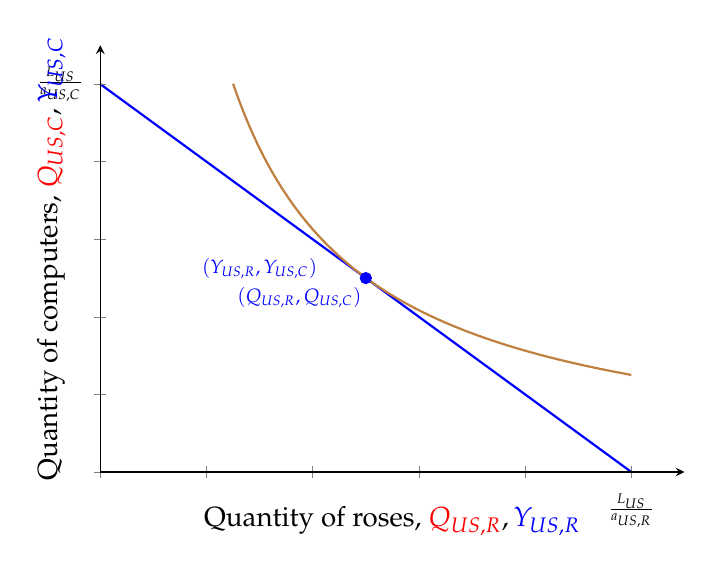
\begin{tikzpicture}
\pgfmathsetmacro{\aC}{100}       % unit labor requirement for computers
\pgfmathsetmacro{\aR}{1}         % unit labor requirement for roses
\pgfmathsetmacro{\alpha}{0.5}    % preference for computers
\pgfmathsetmacro{\Lendow}{10}    % labor endowment

% Compute equilibrium quantities
\pgfmathsetmacro{\Qc}{(\alpha*\Lendow)/\aC}
\pgfmathsetmacro{\Qr}{((1 - \alpha)*\Lendow)/\aR}

% Compute utility level
\pgfmathsetmacro{\U}{(\Qc^(\alpha))*(\Qr^(1 - \alpha))}

% Compute prefactor for indifference curve: Qc = A * Qr^(- (1 - alpha)/alpha)
\pgfmathsetmacro{\expo}{(1 - \alpha)/\alpha}
\pgfmathsetmacro{\A}{\U^(1/\alpha)}

\centering
\begin{axis}[
    ylabel={Quantity of computers, $\textcolor{red}{Q_{US,C}}, \textcolor{blue}{Y_{US,C}}$},
    xlabel={Quantity of roses, $\textcolor{red}{Q_{US,R}}, \textcolor{blue}{Y_{US,R}}$},
    ymin=0, ymax=0.11,
    xmin=0, xmax=11,
    yticklabel=\empty,
    xticklabel=\empty,
    axis lines=left,
    enlargelimits=false,
    clip=false,
    axis on top,
    scaled x ticks=false,
    width=9cm, height=7cm,
    title style={font=\bfseries}
]

% PPF: Q_C = (L/a_C) - (a_R/a_C) * Q_R
\addplot[thick, blue, domain=0:10] {\Lendow/\aC - (\aR/\aC)*x};

% Indifference curve through optimal bundle
\addplot[thick, brown, domain=2.5:10, samples=100] {\A * x^(-\expo)};

% Labels
%\node at (axis cs:3.5,0.03) {\Large $\mathcal{Y}_{US}$};
\node at (axis cs:\Lendow/\aR,-.01) {\scriptsize $\frac{L_{US}}{a_{US,R}}$};
\node at (axis cs:-.75,\Lendow/\aC) {\scriptsize $\frac{L_{US}}{a_{US,C}}$};


% Equilibrium point
\addplot[only marks, mark=*, color=blue, mark size=2pt] coordinates {(\Qr, \Qc)};
\node at (axis cs:\Qr - 1.25,\Qc - 0.005) {\scriptsize $\textcolor{blue}{(Q_{US,R},Q_{US,C})}$};
\node at (axis cs:\Qr - 2,\Qc + 0.0025) {\scriptsize $\textcolor{blue}{(Y_{US,R},Y_{US,C})}$};



\end{axis}

\end{tikzpicture}
}
\end{subfigure}
%
% Colombia
\begin{subfigure}{}
\resizebox{0.48\textwidth}{!}{%

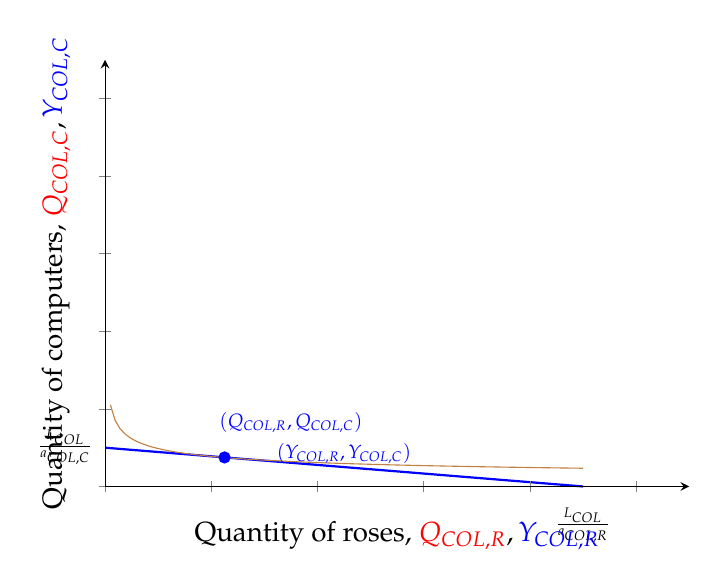
\begin{tikzpicture}
\pgfmathsetmacro{\aC}{900}       % unit labor requirement for computers
\pgfmathsetmacro{\aR}{1}         % unit labor requirement for roses
\pgfmathsetmacro{\alpha}{0.75}    % preference for computers
\pgfmathsetmacro{\Lendow}{9}    % labor endowment

% Compute equilibrium quantities
\pgfmathsetmacro{\Qc}{(\alpha*\Lendow)/\aC}
\pgfmathsetmacro{\Qr}{((1 - \alpha)*\Lendow)/\aR}

% Compute utility level
\pgfmathsetmacro{\U}{(\Qc^(\alpha))*(\Qr^(1 - \alpha))}

% Compute prefactor for indifference curve: Qc = A * Qr^(- (1 - alpha)/alpha)
\pgfmathsetmacro{\expo}{(1 - \alpha)/\alpha}
\pgfmathsetmacro{\A}{\U^(1/\alpha)}

\centering
\begin{axis}[
    ylabel={Quantity of computers, $\textcolor{red}{Q_{COL,C}}, \textcolor{blue}{Y_{COL,C}}$},
    xlabel={Quantity of roses, $\textcolor{red}{Q_{COL,R}}, \textcolor{blue}{Y_{COL,R}}$},
    ymin=0, ymax=0.11,
    xmin=0, xmax=11,
    yticklabel=\empty,
    xticklabel=\empty,
    axis lines=left,
    enlargelimits=false,
    clip=false,
    axis on top,
    scaled x ticks=false,
    width=9cm, height=7cm,
    title style={font=\bfseries}
]

% PPF: Q_C = (L/a_C) - (a_R/a_C) * Q_R
\addplot[thick, blue, domain=0:9] {\Lendow/\aC - (\aR/\aC)*x};

% Indifference curve through optimal bundle
\addplot[brown, domain=0.1:9, samples=100] {\A * x^(-\expo)};

% Labels

%\node at (axis cs:3.5,0.03) {\Large $\mathcal{Y}_{US}$};
\node at (axis cs:\Lendow/\aR,-.01) {\scriptsize $\frac{L_{COL}}{a_{COL,R}}$};
\node at (axis cs:-.75,\Lendow/\aC) {\scriptsize $\frac{L_{COL}}{a_{COL,C}}$};


% Equilibrium point
\addplot[only marks, mark=*, color=blue, mark size=2pt] coordinates {(\Qr, \Qc)};
\node at (axis cs:\Qr + 1.25,\Qc + 0.009) {\scriptsize $\textcolor{blue}{(Q_{COL,R},Q_{COL,C})}$};
\node at (axis cs:\Qr + 2.25,\Qc + 0.001) {\scriptsize $\textcolor{blue}{(Y_{COL,R},Y_{COL,C})}$};


\end{axis}

\end{tikzpicture}
}

\end{subfigure}

\caption{Autarky equilibrium}\label{fig: autarky-num}

\end{figure}


\part Now suppose that countries open up to trade. How would you solve for equilibrium prices under free trade? You don't have to actually solve for them. Just explain your logic.

\textcolor{red}{You would use a global market clearing condition in which total relative demand equals total relative supply (or, equivalently, the value of exports of a given good must be equal to the value of exports of the other good)}.


\part What is the inequality condition for equilibrium prices that allow free trade with specialization to occur? Explain intuitively why that is the case.

\textcolor{red}{    \begin{equation*}\label{eq: price-trade}
        \frac{a_{US,C}}{a_{US,R}} < \frac{P_C}{P_R} < \frac{a_{COL,C}}{a_{COL,R}}
    \end{equation*}}

\textcolor{red}{Trade only happens if it is between domestic opportunity costs (which are also equal to the autarky prices). If prices are equal to opportunity costs, producers will not fully specialize (as they did not in autarky).}


\part Draw the global equilibrium in which world relative demand meets world relative supply, assuming it lays on the trade region. Mark the equilibrium point and explain what happens with production in each country on that region.


\begin{figure}[htpd!]
\centering
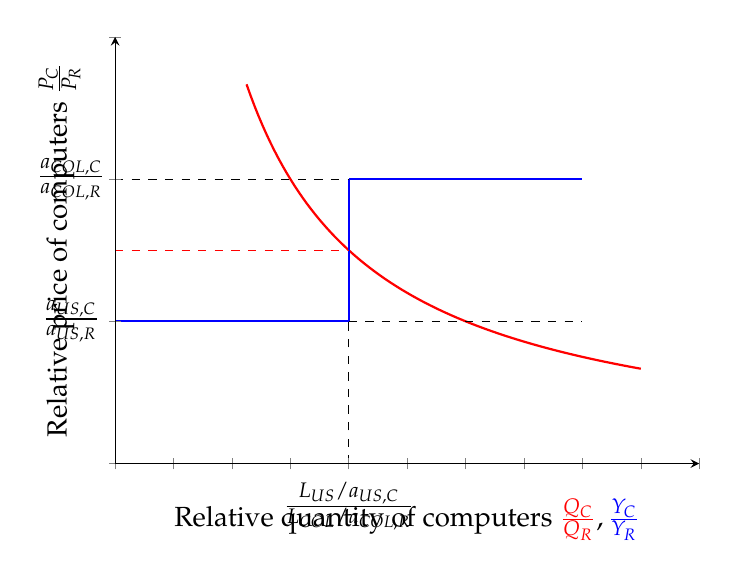
\begin{tikzpicture}
\begin{axis}[
    ylabel={Relative price of computers $\frac{P_C}{P_R}$},
    xlabel={Relative quantity of computers $\textcolor{red}{\frac{Q_{C}}{Q_{R}} } , \textcolor{blue}{\frac{Y_{C}}{Y_{R}} }$},
    ymin=0, ymax=3,
    xmin=0, xmax=2,
    yticklabel=\empty,
    xticklabel=\empty,
    axis lines=left,
    enlargelimits=false,
    clip=false,
    axis on top,
    scaled x ticks=false,
    width=9cm, height=7cm,
    title style={font=\bfseries}]

% Relative Demand RD
\addplot[
    red, thick,
    domain=0.45:1.8,
    samples=100
] {1.2/(x)};
%\node[red] at (axis cs:1.4,1.25) {\small $RD$};

% Relative Supply RS
\addplot[thick, blue] coordinates {(0,1) (0.8,1.0)};
\addplot[thick, blue] coordinates {(0.8,1.0) (0.8,2.0)};
\addplot[thick, blue] coordinates {(0.8,2.0) (1.6,2.0)};
%\node at (axis cs:1.65,2.7) {\small $RS$};

% Dashed lines for autarky prices
\addplot[dashed] coordinates {(0,2.0) (0.8,2.0)};
\node at (axis cs:-0.15,2) {$\frac{a_{COL,C}}{a_{COL,R}}$};

\addplot[dashed] coordinates {(0.8,1.0) (1.6,1.0)};
\node at (axis cs:-0.15,1) {$\frac{a_{US,C}}{a_{US,R}}$};

\addplot[dashed, red] coordinates {(0,1.5) (0.8,1.5)};

% Vertical dashed lines for quantities
\addplot[dashed] coordinates {(0.8,0) (0.8,1.0)};
\node at (axis cs:0.8,-0.3) {$\frac{L_{US}/a_{US,C}}{L_{COL}/a_{COL,R}}$};

\end{axis}
\end{tikzpicture}
\caption{Relative Supply and Demand of Computers as a Function of Relative Prices}
\end{figure}

\textcolor{red}{The vertical segment of the blue line denotes the range for which the inequality above holds -- i.e., the range for which countries will fully specialize in the goods for which they have a comparative advantage.}

\newpage

\part Draw a diagram that shows, for each country, the PPFs; production and consumption in autarky; the new price line (assuming in falls in the traded inducing region); production and consumption under free trade.


\begin{figure}[htbp]

% California
\begin{subfigure}{}
\resizebox{0.48\linewidth}{!}{%
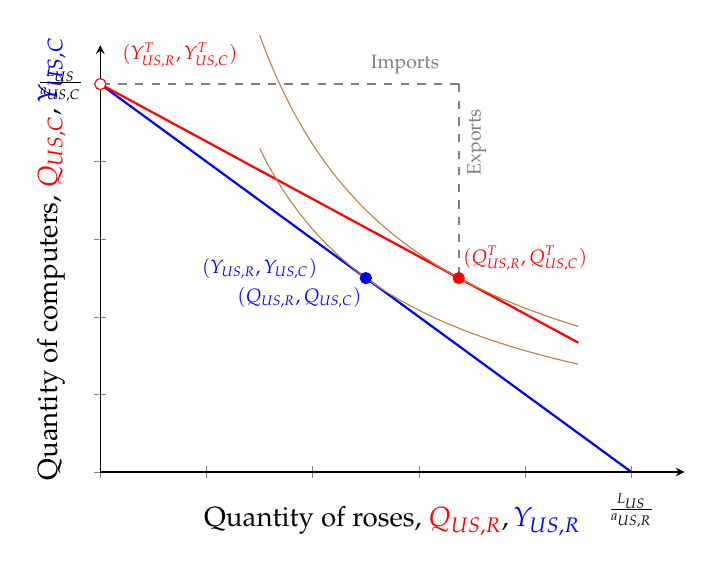
\begin{tikzpicture}
\pgfmathsetmacro{\aC}{100}       % unit labor requirement for computers
\pgfmathsetmacro{\aR}{1}         % unit labor requirement for roses
\pgfmathsetmacro{\alpha}{0.5}    % preference for computers
\pgfmathsetmacro{\Lendow}{10}    % labor endowment
\pgfmathsetmacro{\p}{135}    % trade price

% Compute equilibrium quantities
\pgfmathsetmacro{\Qc}{(\alpha*\Lendow)/\aC}
\pgfmathsetmacro{\Qr}{((1 - \alpha)*\Lendow)/\aR}
\pgfmathsetmacro{\QcT}{(\alpha*\Lendow)/\aC}
\pgfmathsetmacro{\QrT}{((1 - \alpha)*\p*\Lendow)/\aC}

% Compute utility level
\pgfmathsetmacro{\U}{(\Qc^(\alpha))*(\Qr^(1 - \alpha))}
\pgfmathsetmacro{\UT}{(\QcT^(\alpha))*(\QrT^(1 - \alpha))}

% Compute prefactor for indifference curve: Qc = A * Qr^(- (1 - alpha)/alpha)
\pgfmathsetmacro{\expo}{(1 - \alpha)/\alpha}
\pgfmathsetmacro{\A}{\U^(1/\alpha)}
\pgfmathsetmacro{\AT}{\UT^(1/\alpha)}

\centering
\begin{axis}[
    ylabel={Quantity of computers, $\textcolor{red}{Q_{US,C}}, \textcolor{blue}{Y_{US,C}}$},
    xlabel={Quantity of roses, $\textcolor{red}{Q_{US,R}}, \textcolor{blue}{Y_{US,R}}$},
    ymin=0, ymax=\Lendow/\aC * 1.1,
    xmin=0, xmax=\Lendow/\aR * 1.1,
    yticklabel=\empty,
    xticklabel=\empty,
    axis lines=left,
    enlargelimits=false,
    clip=false,
    axis on top,
    scaled x ticks=false,
    width=9cm, height=7cm,
    title style={font=\bfseries}
]

% PPF: Q_C = (L/a_C) - (a_R/a_C) * Q_R
\addplot[thick, blue, domain=0:10] {\Lendow/\aC - (\aR/\aC)*x};
\addplot[thick, red, domain=0:9] {\Lendow/\aC  - (1/\p)*x};

% Indifference curve through optimal bundle
\addplot[brown, domain=3:9, samples=100] {\A * x^(-\expo)};
\addplot[brown, domain=3:9, samples=100] {\AT * x^(-\expo)};

% Labels

%\node at (axis cs:3.5,0.03) {\Large $\mathcal{Y}_{US}$};
\node at (axis cs:\Lendow/\aR,-.01) {\scriptsize $\frac{L_{US}}{a_{US,R}}$};
\node at (axis cs:-.75,\Lendow/\aC) {\scriptsize $\frac{L_{US}}{a_{US,C}}$};

% Equilibrium point
\addplot[only marks, mark=*, color=blue, mark size=2pt] coordinates {(\Qr, \Qc)};
\node at (axis cs:\Qr - 1.25,\Qc - 0.005) {\scriptsize $\textcolor{blue}{(Q_{US,R},Q_{US,C})}$};
\node at (axis cs:\Qr - 2,\Qc + 0.0025) {\scriptsize $\textcolor{blue}{(Y_{US,R},Y_{US,C})}$};

\addplot[only marks, mark=*, color=red, mark size=2pt] coordinates {(\QrT, \QcT)};
\node at (axis cs:\QrT + 1.25,\QcT + 0.005) {\scriptsize $\textcolor{red}{(Q^T_{US,R},Q^T_{US,C})}$};

\addplot[only marks, mark=*, mark options={fill=white, draw=red}, mark size=2pt] coordinates {(0, \Lendow/\aC)};
\node at (axis cs:0 + 1.5,\Lendow/\aC + 0.0075) {\scriptsize $\textcolor{red}{(Y^T_{US,R},Y^T_{US,C})}$};

% Arrows for exports (horizontal)
\draw[-, dashed, thick, gray] 
    (axis cs:\QrT,\Lendow/\aC) -- 
    (axis cs:0,\Lendow/\aC);
\node[gray] at (axis cs:\QrT*0.85,\Lendow/\aC*1.05) {\scriptsize Imports};

% Arrows for imports (vertical)
\draw[-, dashed, thick, gray] 
    (axis cs:\QrT,\Lendow/\aC) -- 
    (axis cs:\QrT, \QcT);
\node[gray, rotate=90] at (axis cs:\QrT*1.05,\Lendow/\aC*0.85) {\scriptsize Exports};



\end{axis}

\end{tikzpicture}
}
\end{subfigure}
%
% Colombia
\begin{subfigure}{}
\resizebox{0.48\linewidth}{!}{%

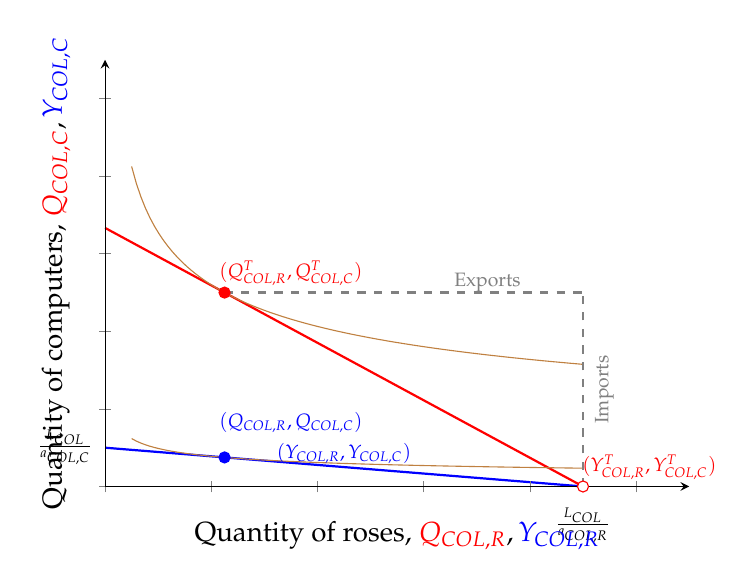
\begin{tikzpicture}
\pgfmathsetmacro{\aC}{900}       % unit labor requirement for computers
\pgfmathsetmacro{\aR}{1}         % unit labor requirement for roses
\pgfmathsetmacro{\alpha}{0.75}    % preference for computers
\pgfmathsetmacro{\Lendow}{9}    % labor endowment
\pgfmathsetmacro{\p}{135}    % trade price


% Compute equilibrium quantities
\pgfmathsetmacro{\Qc}{(\alpha*\Lendow)/\aC}
\pgfmathsetmacro{\Qr}{((1 - \alpha)*\Lendow)/\aR}
\pgfmathsetmacro{\QcT}{(\alpha*\Lendow)/(\aR*\p)}
\pgfmathsetmacro{\QrT}{((1 - \alpha)*\Lendow)/\aR}

% Compute prefactor for indifference curve: Qc = A * Qr^(- (1 - alpha)/alpha)
\pgfmathsetmacro{\expo}{(1 - \alpha)/\alpha}
\pgfmathsetmacro{\A}{\Qc * \Qr^((1 - \alpha)/\alpha))}
\pgfmathsetmacro{\AT}{\QcT * \QrT^((1 - \alpha)/\alpha))}

\centering
\begin{axis}[
    ylabel={Quantity of computers, $\textcolor{red}{Q_{COL,C}}, \textcolor{blue}{Y_{COL,C}}$},
    xlabel={Quantity of roses, $\textcolor{red}{Q_{COL,R}}, \textcolor{blue}{Y_{COL,R}}$},
    ymin=0, ymax=0.11,
    xmin=0, xmax=11,
    yticklabel=\empty,
    xticklabel=\empty,
    axis lines=left,
    enlargelimits=false,
    clip=false,
    axis on top,
    scaled x ticks=false,
    width=9cm, height=7cm,
    title style={font=\bfseries}
]

% PPF: Q_C = (L/a_C) - (a_R/a_C) * Q_R
\addplot[thick, blue, domain=0:9] {\Lendow/\aC - (\aR/\aC)*x};
\addplot[thick, red, domain=0:9] {\Lendow/\aR * 1/ \p - (1/\p)*x};


% Indifference curve through optimal bundle
\addplot[brown, domain=0.5:9, samples=100] {\A * x^(-\expo)};
\addplot[brown, domain=0.5:9, samples=100] {\AT * x^(-\expo)};

% Labels

%\node at (axis cs:3.5,0.03) {\Large $\mathcal{Y}_{US}$};
\node at (axis cs:\Lendow/\aR,-.01) {\scriptsize $\frac{L_{COL}}{a_{COL,R}}$};
\node at (axis cs:-.75,\Lendow/\aC) {\scriptsize $\frac{L_{COL}}{a_{COL,C}}$};


% Equilibrium point
\addplot[only marks, mark=*, color=blue, mark size=2pt] coordinates {(\Qr, \Qc)};
\node at (axis cs:\Qr + 1.25,\Qc + 0.009) {\scriptsize $\textcolor{blue}{(Q_{COL,R},Q_{COL,C})}$};
\node at (axis cs:\Qr + 2.25,\Qc + 0.001) {\scriptsize $\textcolor{blue}{(Y_{COL,R},Y_{COL,C})}$};


\addplot[only marks, mark=*, color=red, mark size=2pt] coordinates {(\QrT, \QcT)};
\node at (axis cs:\QrT + 1.25,\QcT + 0.005) {\scriptsize $\textcolor{red}{(Q^T_{COL,R},Q^T_{COL,C})}$};

\addplot[only marks, mark=*, mark options={fill=white, draw=red}, mark size=2pt] coordinates {(\Lendow/\aR, 0)};
\node at (axis cs:\Lendow/\aR + 1.25,0 + 0.005) {\scriptsize $\textcolor{red}{(Y^T_{COL,R},Y^T_{COL,C})}$};

% Arrows for exports (horizontal)
\draw[-, dashed, thick, gray] 
    (axis cs:\QrT,\QcT) -- 
    (axis cs:\Lendow/\aR,\QcT);
\node[gray] at (axis cs:{ \Lendow/\aR *0.8}, \QcT*1.05) {\scriptsize Exports};

% Arrows for imports (vertical)
\draw[-, dashed, thick, gray] 
    (axis cs:{\Lendow/\aR},0) -- 
    (axis cs:{\Lendow/\aR}, \QcT);
\node[gray, rotate=90] at (axis cs:{\Lendow/\aR + 0.4}, {\QcT/2}) {\scriptsize Imports};

\end{axis}

\end{tikzpicture}
}

\end{subfigure}

\caption{Specialization + Trade Equilibrium}

\end{figure}


\end{parts}

\question Home has 1,200 units of labor available. It can produce two goods, apples and bananas. The unit labor requirement in apple production is 3, while in banana
production it is 2.
\begin{parts}
\part Graph Home’s production possibility frontier.

    \textcolor{red}{
    \begin{align*}
        a_{H,Apple} Y_{H,Apple} + a_{H,Banana} Y_{H,Banana} = L_{h} \\
        3 Y_{H,Apple} + 2 Y_{H,Banana} = 1200 \\
         Y_{H,Apple} = 1200/3  - 2/3 Y_{H,Banana} \\
         Y_{H,Apple} = 400  - 2/3 Y_{H,Banana}
   \end{align*}
    }

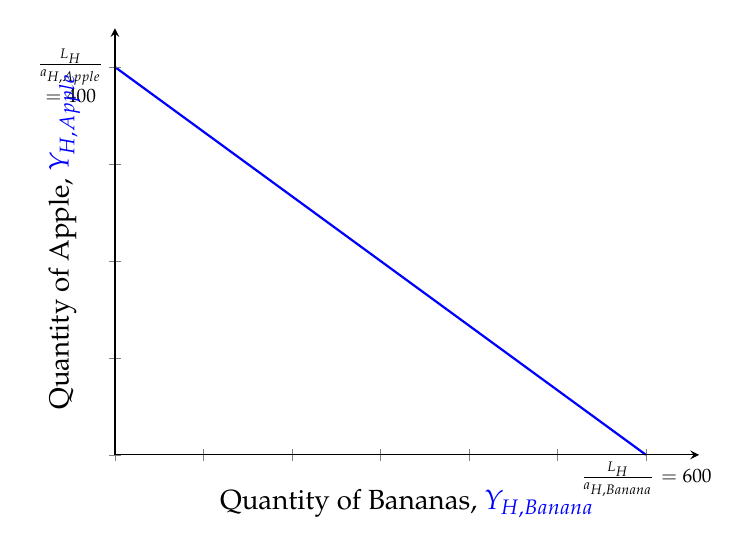
\begin{tikzpicture}
\pgfmathsetmacro{\aC}{3}       % unit labor requirement for computers
\pgfmathsetmacro{\aR}{2}         % unit labor requirement for roses
\pgfmathsetmacro{\Lendow}{1200}    % labor endowment

\centering
\begin{axis}[
    ylabel={Quantity of Apple, $\textcolor{blue}{Y_{H,Apple}}$},
    xlabel={Quantity of Bananas, $\textcolor{blue}{Y_{H,Banana}}$},
    ymin=0, ymax=\Lendow/\aC * 1.1,
    xmin=0, xmax=\Lendow/\aR * 1.1,
    yticklabel=\empty,
    xticklabel=\empty,
    axis lines=left,
    enlargelimits=false,
    clip=false,
    axis on top,
    scaled x ticks=false,
    width=9cm, height=7cm,
    title style={font=\bfseries}
]

% PPF: Q_C = (L/a_C) - (a_R/a_C) * Q_R
\addplot[thick, blue, domain=0:\Lendow/\aR] {\Lendow/\aC - (\aR/\aC)*x};

%\node at (axis cs:3.5,0.03) {\Large $\mathcal{Y}_{US}$};
\node at (axis cs:\Lendow/\aR,-25) {\scriptsize $\frac{L_{H}}{a_{H,Banana}}=600$};
\node at (axis cs:-50,\Lendow/\aC) {\scriptsize $\frac{L_{H}}{a_{H,Apple}}$};
\node at (axis cs:-50,\Lendow/\aC-30) {\scriptsize $=400$};



\end{axis}

\end{tikzpicture}

\part What is the opportunity cost of apples in terms of bananas? 

\begin{align*}
\red{
    a_{H,Banana}/a_{H,Apple} = 2/3  \text{ (or equivalently) } a_{H,Apple}/a_{H,Banana} = 3/2
}
\end{align*}


\part In the absence of trade, what would be the price of apples in terms of bananas? Why?
\red{ In the absence of trade, relative prices reflect opportunity costs:
\begin{align*}
    P_{Banana}/P_{Apple} = a_{H,Banana}/a_{H,Apple} = 2/3 \text{ (or equivalently) } \\ P_{Apple}/P_{Banana} = a_{H,Apple}/a_{H,Banana} = 3/2
\end{align*}
}
\end{parts}

\question Home is as described above. There is now also another country, Foreign,
with a labor force of 800. Foreign’s unit labor requirement in apple production
is 5, while in banana production it is 1.
\begin{parts}
    \item Graph Foreign’s production possibility frontier.

    \textcolor{red}{
    \begin{align*}
        a_{F,Apple} Y_{F,Apple} + a_{F,Banana} Y_{F,Banana} \leq L_{F} \\
        5 Y_{F,Apple} + 1 Y_{F,Banana} \leq 800
    \end{align*}
    }
    \textcolor{red}{
    The PPF is a straight line connecting the intercepts:
    \begin{itemize}
        \item If all labor is in apples: $Y_{F,Apple} = 800/5 = 160$, $Y_{F,Banana} = 0$
        \item If all labor is in bananas: $Y_{F,Banana} = 800/1 = 800$, $Y_{F,Apple} = 0$
    \end{itemize}
    The slope of the PPF (opportunity cost of apples): $-a_{F,Apple}/a_{F,Banana} = -5$ (or) $-a_{F,Banana}/a_{F,Apple} = -1/5$ depending on which variable you plot on the y axis.
    }


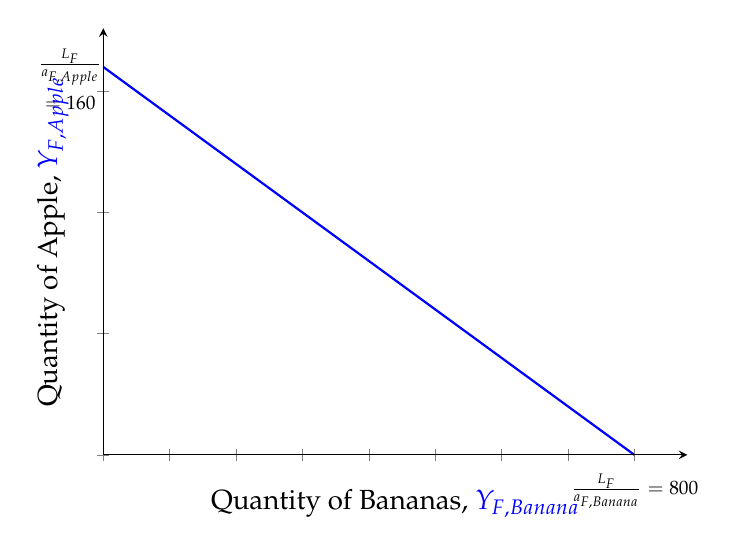
\begin{tikzpicture}
\pgfmathsetmacro{\aC}{5}       % unit labor requirement for computers
\pgfmathsetmacro{\aR}{1}         % unit labor requirement for roses
\pgfmathsetmacro{\Lendow}{800}    % labor endowment

\centering
\begin{axis}[
    ylabel={Quantity of Apple, $\textcolor{blue}{Y_{F,Apple}}$},
    xlabel={Quantity of Bananas, $\textcolor{blue}{Y_{F,Banana}}$},
    ymin=0, ymax=\Lendow/\aC * 1.1,
    xmin=0, xmax=\Lendow/\aR * 1.1,
    yticklabel=\empty,
    xticklabel=\empty,
    axis lines=left,
    enlargelimits=false,
    clip=false,
    axis on top,
    scaled x ticks=false,
    width=9cm, height=7cm,
    title style={font=\bfseries}
]

% PPF: Q_C = (L/a_C) - (a_R/a_C) * Q_R
\addplot[thick, blue, domain=0:\Lendow/\aR] {\Lendow/\aC - (\aR/\aC)*x};

%\node at (axis cs:3.5,0.03) {\Large $\mathcal{Y}_{US}$};
\node at (axis cs:\Lendow/\aR,-15) {\scriptsize $\frac{L_{F}}{a_{F,Banana}}=800$};
\node at (axis cs:-50,\Lendow/\aC) {\scriptsize $\frac{L_{F}}{a_{F,Apple}}$};
\node at (axis cs:-50,\Lendow/\aC-15) {\scriptsize $=160$};



\end{axis}

\end{tikzpicture}

    \item Construct the world relative supply curve.

    \textcolor{red}{
    For both countries, calculate maximum output if specializing:
    \begin{align*}
        \text{Home:} &\quad Y_{H,Apple} = 400,\, Y_{H,Banana} = 600 \\
        \text{Foreign:} &\quad Y_{F,Apple} = 160,\, Y_{F,Banana} = 800
    \end{align*}
    }
    \textcolor{red}{
    The world relative supply (RS) curve is stepwise:
    \begin{itemize}
        \item When $P_{Apple}/P_{Banana} < $ Home's opportunity cost ($a_{H,Apple}/a_{H,Banana}=3/2=1.5$), both countries specialize in bananas. RS is lowest.
        \item When $1.5 < P_{Apple}/P_{Banana} < 5$ (Foreign's opportunity cost), Home specializes in apples, Foreign in bananas.
        \item When $P_{Apple}/P_{Banana} > 5$, both specialize in apples. RS is highest.
    \end{itemize}
    }

    \begin{figure}[htpd!]
\centering
\begin{tikzpicture}
\begin{axis}[
    ylabel={Relative price of apples $\frac{P_{Apple}}{P_{Banana}}$},
    xlabel={Relative quantity of apples $ \textcolor{blue}{\frac{Y_{Apple}}{Y_{Banana}} }$$},
    ymin=0, ymax=6,
    xmin=0, xmax=1,
    yticklabel=\empty,
    xticklabel=\empty,
    axis lines=left,
    enlargelimits=false,
    clip=false,
    axis on top,
    scaled x ticks=false,
    width=9cm, height=7cm,
    title style={font=\bfseries}]


% Relative Supply RS
\addplot[thick, blue] coordinates {(0,3/2) (1/2,3/2)};
\addplot[thick, blue] coordinates {(1/2,3/2) (1/2,5)};
\addplot[thick, blue] coordinates {(1/2,5) (1,5)};
%\node at (axis cs:1.65,2.7) {\small $RS$};

% Dashed lines for autarky prices
\addplot[dashed] coordinates {(0,5) (1/2,5)};
\node at (axis cs:-.05,5) {$5$};

\addplot[dashed] coordinates {(1/2,3/2) (1,3/2)};
\node at (axis cs:-.05,3/2) {$3/2$};


% Vertical dashed lines for quantities
\addplot[dashed] coordinates {(1/2,0) (1/2,3/2)};
\node at (axis cs:1/2,-0.3) {$\frac{400}{800} = 1/2$};

\end{axis}
\end{tikzpicture}
\end{figure}


\end{parts}

\question Now suppose world relative demand takes the following form: Demand for apples/demand for bananas = price of bananas/price of apples.
\begin{parts}
\part Graph the relative demand curve along with the relative supply curve.

\textcolor{red}{
Relative Demand (RD):
\begin{align*}
    \frac{Q_{Apple}}{Q_{Banana}} = \frac{P_{Banana}}{P_{Apple}} = \frac{1}{P_{Apple}/P_{Banana}}
\end{align*}
\red{
This is a downward sloping curve, showing that as $P_{Apple}/P_{Banana}$ rises, $Q_{Apple}^D/Q_{Banana}^D$ falls.
}
\textcolor{red}{
\begin{itemize}
    \item On the same axes, plot RS (stepwise) and RD (downward sloping).
    \item The intersection determines equilibrium.
\end{itemize}
}
}

    \begin{figure}[htpd!]
\centering
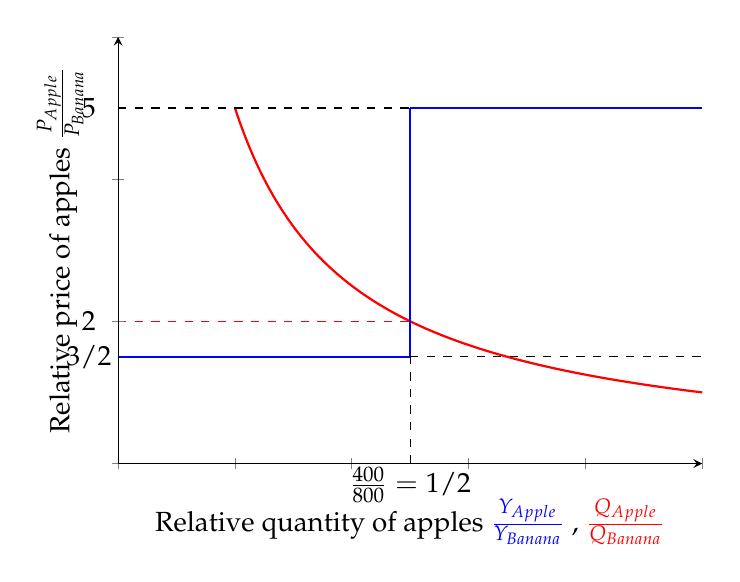
\begin{tikzpicture}
\begin{axis}[
    ylabel={Relative price of apples $\frac{P_{Apple}}{P_{Banana}}$},
    xlabel={Relative quantity of apples $ \textcolor{blue}{\frac{Y_{Apple}}{Y_{Banana}} }$ , $\red{\frac{Q_{Apple}}{Q_{Banana}}}$},
    ymin=0, ymax=6,
    xmin=0, xmax=1,
    yticklabel=\empty,
    xticklabel=\empty,
    axis lines=left,
    enlargelimits=false,
    clip=false,
    axis on top,
    scaled x ticks=false,
    width=9cm, height=7cm,
    title style={font=\bfseries}]

% Relative Demand RD
\addplot[
    red, thick,
    domain=0.2:1,
    samples=100
] {1/(x)};
\addplot[dashed, red] coordinates {(0,2) (1/2,2)};
\node at (axis cs:-.05,2) {$2$};

% Relative Supply RS
\addplot[thick, blue] coordinates {(0,3/2) (1/2,3/2)};
\addplot[thick, blue] coordinates {(1/2,3/2) (1/2,5)};
\addplot[thick, blue] coordinates {(1/2,5) (1,5)};
%\node at (axis cs:1.65,2.7) {\small $RS$};

% Dashed lines for autarky prices
\addplot[dashed] coordinates {(0,5) (1/2,5)};
\node at (axis cs:-.05,5) {$5$};

\addplot[dashed] coordinates {(1/2,3/2) (1,3/2)};
\node at (axis cs:-.05,3/2) {$3/2$};


% Vertical dashed lines for quantities
\addplot[dashed] coordinates {(1/2,0) (1/2,3/2)};
\node at (axis cs:1/2,-0.3) {$\frac{400}{800} = 1/2$};

\end{axis}
\end{tikzpicture}
\end{figure}

\part What is the equilibrium relative price of apples?

\textcolor{red}{
The equilibrium occurs where world relative supply equals world relative demand:
\begin{align*}
    RS = RD \implies \frac{Y_{Apple}^{World}}{Y_{Banana}^{World}} = \frac{P_{Banana}}{P_{Apple}}
\end{align*}
At the kink in RS (where Home specializes in apples, Foreign in bananas): 
\begin{align*}
    Y_{Apple}^{World} = 400 \quad Y_{Banana}^{World} = 800 \\
    RS = 400/800 = 0.5 \\
    RD = P_{Banana}/P_{Apple} = 0.5 \implies P_{Apple}/P_{Banana} = 2
\end{align*}
So equilibrium relative price: $P_{Apple}/P_{Banana} = 2$
}

\part Describe the pattern of trade.

\textcolor{red}{
\begin{itemize}
    \item Home specializes in apples and exports apples to Foreign.
    \item Foreign specializes in bananas and exports bananas to Home.
    \item Each country imports the good for which it does not have a comparative advantage.
\end{itemize}
}

\part Show that both Home and Foreign gain from trade.

\textcolor{red}{
Under autarky, each country consumes on its PPF, at its own opportunity cost. With trade:
\begin{itemize}
    \item Both can consume bundles outside their PPFs (along the international price line).
    \item Both access more of both goods for the same labor input.
    \item This is shown by indifference curves tangent to the trade line above the PPF (draw it).
\end{itemize}
}


\begin{figure}[htbp]

% California
\begin{subfigure}{}
\resizebox{0.48\linewidth}{!}{%
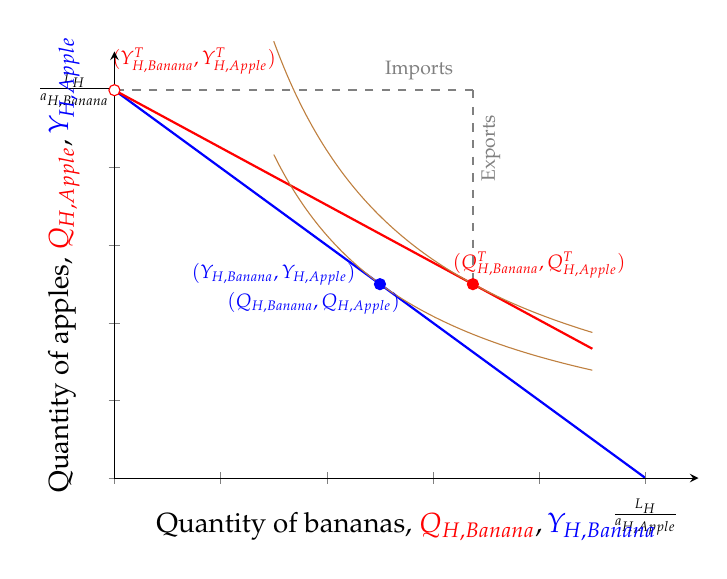
\begin{tikzpicture}
\pgfmathsetmacro{\aC}{100}       % unit labor requirement for computers
\pgfmathsetmacro{\aR}{1}         % unit labor requirement for roses
\pgfmathsetmacro{\alpha}{0.5}    % preference for computers
\pgfmathsetmacro{\Lendow}{10}    % labor endowment
\pgfmathsetmacro{\p}{135}    % trade price

% Compute equilibrium quantities
\pgfmathsetmacro{\Qc}{(\alpha*\Lendow)/\aC}
\pgfmathsetmacro{\Qr}{((1 - \alpha)*\Lendow)/\aR}
\pgfmathsetmacro{\QcT}{(\alpha*\Lendow)/\aC}
\pgfmathsetmacro{\QrT}{((1 - \alpha)*\p*\Lendow)/\aC}

% Compute utility level
\pgfmathsetmacro{\U}{(\Qc^(\alpha))*(\Qr^(1 - \alpha))}
\pgfmathsetmacro{\UT}{(\QcT^(\alpha))*(\QrT^(1 - \alpha))}

% Compute prefactor for indifference curve: Qc = A * Qr^(- (1 - alpha)/alpha)
\pgfmathsetmacro{\expo}{(1 - \alpha)/\alpha}
\pgfmathsetmacro{\A}{\U^(1/\alpha)}
\pgfmathsetmacro{\AT}{\UT^(1/\alpha)}

\centering
\begin{axis}[
    ylabel={Quantity of apples, $\textcolor{red}{Q_{H,Apple}}, \textcolor{blue}{Y_{H,Apple}}$},
    xlabel={Quantity of bananas, $\textcolor{red}{Q_{H,Banana}}, \textcolor{blue}{Y_{H,Banana}}$},
    ymin=0, ymax=\Lendow/\aC * 1.1,
    xmin=0, xmax=\Lendow/\aR * 1.1,
    yticklabel=\empty,
    xticklabel=\empty,
    axis lines=left,
    enlargelimits=false,
    clip=false,
    axis on top,
    scaled x ticks=false,
    width=9cm, height=7cm,
    title style={font=\bfseries}
]

% PPF: Q_C = (L/a_C) - (a_R/a_C) * Q_R
\addplot[thick, blue, domain=0:10] {\Lendow/\aC - (\aR/\aC)*x};
\addplot[thick, red, domain=0:9] {\Lendow/\aC  - (1/\p)*x};

% Indifference curve through optimal bundle
\addplot[brown, domain=3:9, samples=100] {\A * x^(-\expo)};
\addplot[brown, domain=3:9, samples=100] {\AT * x^(-\expo)};

% Labels

%\node at (axis cs:3.5,0.03) {\Large $\mathcal{Y}_{US}$};
\node at (axis cs:\Lendow/\aR,-.01) {\scriptsize $\frac{L_{H}}{a_{H,Apple}}$};
\node at (axis cs:-.75,\Lendow/\aC) {\scriptsize $\frac{L_{H}}{a_{H,Banana}}$};

% Equilibrium point
\addplot[only marks, mark=*, color=blue, mark size=2pt] coordinates {(\Qr, \Qc)};
\node at (axis cs:\Qr - 1.25,\Qc - 0.005) {\scriptsize $\textcolor{blue}{(Q_{H,Banana},Q_{H,Apple})}$};
\node at (axis cs:\Qr - 2,\Qc + 0.0025) {\scriptsize $\textcolor{blue}{(Y_{H,Banana},Y_{H,Apple})}$};

\addplot[only marks, mark=*, color=red, mark size=2pt] coordinates {(\QrT, \QcT)};
\node at (axis cs:\QrT + 1.25,\QcT + 0.005) {\scriptsize $\textcolor{red}{(Q^T_{H,Banana},Q^T_{H,Apple})}$};

\addplot[only marks, mark=*, mark options={fill=white, draw=red}, mark size=2pt] coordinates {(0, \Lendow/\aC)};
\node at (axis cs:0 + 1.5,\Lendow/\aC + 0.0075) {\scriptsize $\textcolor{red}{(Y^T_{H,Banana},Y^T_{H,Apple})}$};

% Arrows for exports (horizontal)
\draw[-, dashed, thick, gray] 
    (axis cs:\QrT,\Lendow/\aC) -- 
    (axis cs:0,\Lendow/\aC);
\node[gray] at (axis cs:\QrT*0.85,\Lendow/\aC*1.05) {\scriptsize Imports};

% Arrows for imports (vertical)
\draw[-, dashed, thick, gray] 
    (axis cs:\QrT,\Lendow/\aC) -- 
    (axis cs:\QrT, \QcT);
\node[gray, rotate=90] at (axis cs:\QrT*1.05,\Lendow/\aC*0.85) {\scriptsize Exports};



\end{axis}

\end{tikzpicture}
}
\end{subfigure}
%
% Colombia
\begin{subfigure}{}
\resizebox{0.48\linewidth}{!}{%

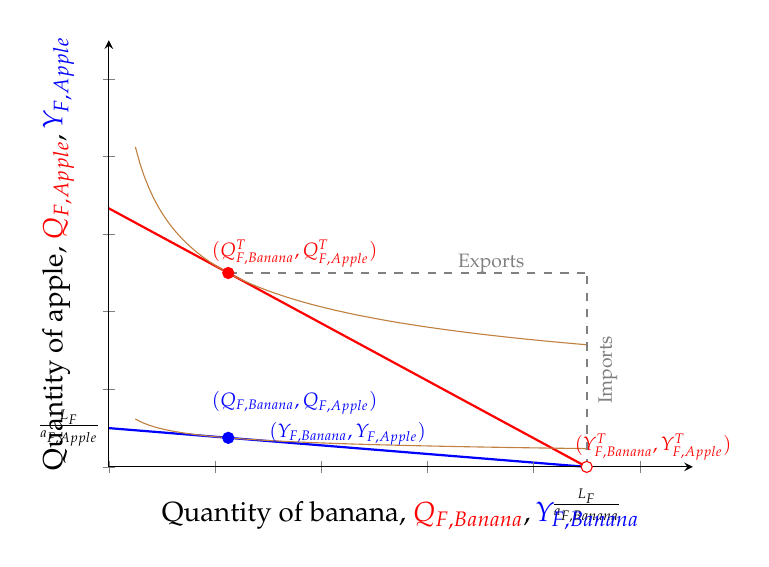
\begin{tikzpicture}
\pgfmathsetmacro{\aC}{900}       % unit labor requirement for computers
\pgfmathsetmacro{\aR}{1}         % unit labor requirement for roses
\pgfmathsetmacro{\alpha}{0.75}    % preference for computers
\pgfmathsetmacro{\Lendow}{9}    % labor endowment
\pgfmathsetmacro{\p}{135}    % trade price


% Compute equilibrium quantities
\pgfmathsetmacro{\Qc}{(\alpha*\Lendow)/\aC}
\pgfmathsetmacro{\Qr}{((1 - \alpha)*\Lendow)/\aR}
\pgfmathsetmacro{\QcT}{(\alpha*\Lendow)/(\aR*\p)}
\pgfmathsetmacro{\QrT}{((1 - \alpha)*\Lendow)/\aR}

% Compute prefactor for indifference curve: Qc = A * Qr^(- (1 - alpha)/alpha)
\pgfmathsetmacro{\expo}{(1 - \alpha)/\alpha}
\pgfmathsetmacro{\A}{\Qc * \Qr^((1 - \alpha)/\alpha))}
\pgfmathsetmacro{\AT}{\QcT * \QrT^((1 - \alpha)/\alpha))}

\centering
\begin{axis}[
    ylabel={Quantity of apple, $\textcolor{red}{Q_{F,Apple}}, \textcolor{blue}{Y_{F,Apple}}$},
    xlabel={Quantity of banana, $\textcolor{red}{Q_{F,Banana}}, \textcolor{blue}{Y_{F,Banana}}$},
    ymin=0, ymax=0.11,
    xmin=0, xmax=11,
    yticklabel=\empty,
    xticklabel=\empty,
    axis lines=left,
    enlargelimits=false,
    clip=false,
    axis on top,
    scaled x ticks=false,
    width=9cm, height=7cm,
    title style={font=\bfseries}
]

% PPF: Q_C = (L/a_C) - (a_R/a_C) * Q_R
\addplot[thick, blue, domain=0:9] {\Lendow/\aC - (\aR/\aC)*x};
\addplot[thick, red, domain=0:9] {\Lendow/\aR * 1/ \p - (1/\p)*x};


% Indifference curve through optimal bundle
\addplot[brown, domain=0.5:9, samples=100] {\A * x^(-\expo)};
\addplot[brown, domain=0.5:9, samples=100] {\AT * x^(-\expo)};

% Labels

%\node at (axis cs:3.5,0.03) {\Large $\mathcal{Y}_{US}$};
\node at (axis cs:\Lendow/\aR,-.01) {\scriptsize $\frac{L_{F}}{a_{F,Banana}}$};
\node at (axis cs:-.75,\Lendow/\aC) {\scriptsize $\frac{L_{F}}{a_{F,Apple}}$};


% Equilibrium point
\addplot[only marks, mark=*, color=blue, mark size=2pt] coordinates {(\Qr, \Qc)};
\node at (axis cs:\Qr + 1.25,\Qc + 0.009) {\scriptsize $\textcolor{blue}{(Q_{F,Banana},Q_{F,Apple})}$};
\node at (axis cs:\Qr + 2.25,\Qc + 0.001) {\scriptsize $\textcolor{blue}{(Y_{F,Banana},Y_{F,Apple})}$};


\addplot[only marks, mark=*, color=red, mark size=2pt] coordinates {(\QrT, \QcT)};
\node at (axis cs:\QrT + 1.25,\QcT + 0.005) {\scriptsize $\textcolor{red}{(Q^T_{F,Banana},Q^T_{F,Apple})}$};

\addplot[only marks, mark=*, mark options={fill=white, draw=red}, mark size=2pt] coordinates {(\Lendow/\aR, 0)};
\node at (axis cs:\Lendow/\aR + 1.25,0 + 0.005) {\scriptsize $\textcolor{red}{(Y^T_{F,Banana},Y^T_{F,Apple})}$};

% Arrows for exports (horizontal)
\draw[-, dashed, thick, gray] 
    (axis cs:\QrT,\QcT) -- 
    (axis cs:\Lendow/\aR,\QcT);
\node[gray] at (axis cs:{ \Lendow/\aR *0.8}, \QcT*1.05) {\scriptsize Exports};

% Arrows for imports (vertical)
\draw[-, dashed, thick, gray] 
    (axis cs:{\Lendow/\aR},0) -- 
    (axis cs:{\Lendow/\aR}, \QcT);
\node[gray, rotate=90] at (axis cs:{\Lendow/\aR + 0.4}, {\QcT/2}) {\scriptsize Imports};

\end{axis}

\end{tikzpicture}
}

\end{subfigure}

\caption{Specialization + Trade Equilibrium}

\end{figure}

\end{parts}

\question Suppose in an hour, 10 kg of rice and 5 meter of cloth is produced in India, and 5 kg and 2 meter in Thailand. Using opportunity costs, explain which country should export cloth and which should export rice.

\textcolor{red}{
Opportunity cost:
\begin{itemize}
    \item India: 1 cloth = 2 rice ($10/5$), 1 rice = 0.5 cloth
    \item Thailand: 1 cloth = 2.5 rice ($5/2$), 1 rice = 0.4 cloth
\end{itemize}
India has lower opportunity cost in rice, Thailand in cloth.
\textbf{Thus:} India should export rice, Thailand should export cloth (each exports the good for which it has comparative advantage).
}

\question Suppose Mike and Johnson produce two products—hamburgers and T-shirts. Mike
produces 10 hamburgers or 3 T-shirts a day and Johnson produces 7 hamburgers or
4 T-shirts. Assuming they can devote time to making either hamburgers or T-shirts.
\begin{parts}
\part Draw the production possibility curve.

\textcolor{red}{
\begin{itemize}
    \item Mike: PPF from $(10,0)$ to $(0,3)$, slope $-10/3 \approx -3.33$
    \item Johnson: PPF from $(7,0)$ to $(0,4)$, slope $-7/4 = -1.75$
\end{itemize}
Plot both as straight lines connecting the intercepts.
}

\part Who enjoys the absolute advantage of producing both?

\textcolor{red}{
Mike can produce more hamburgers (10 vs 7), but fewer T-shirts (3 vs 4). \\
Johnson has absolute advantage in T-shirts, Mike in hamburgers.
}

\part  Who has a higher opportunity cost of making T-shirts?

\textcolor{red}{
Opportunity cost of 1 T-shirt:
\begin{itemize}
    \item Mike: $10/3 \approx 3.33$ hamburgers per T-shirt.
    \item Johnson: $7/4 = 1.75$ hamburgers per T-shirt.
\end{itemize}
Mike has higher opportunity cost of making T-shirts.
}

\part  \textcolor{red}{Who has a comparative advantage in producing hamburgers?}

\textcolor{red}{
Mike: Opportunity cost of 1 hamburger is $3/10 = 0.3$ T-shirt. \\
Johnson: Opportunity cost of 1 hamburger is $4/7 \approx 0.57$ T-shirt. \\
Mike has lower opportunity cost, so Mike has comparative advantage in hamburgers.
}
\end{parts}

\question It has been \textbf{all downhill for the West since China entered the world market}; we just can’t compete with hundreds of millions of people willing to work for almost nothing. Discuss.

\textcolor{red}{
This statement ignores the principle of comparative advantage. Even if China has a lower cost of production (absolute advantage) in many goods, trade allows all countries to specialize and benefit:
\begin{itemize}
    \item Consumers in the West gain access to cheaper goods.
    \item Resources in the West shift to industries with greater comparative advantage.
    \item Trade increases overall welfare and efficiency.
    \item Short-run adjustment costs exist, but long-run gains from trade are widely supported by economic theory.
\end{itemize}
}

\question In China, local governments are responsible for setting the minimum wages. In the United States, a network of federal laws, state laws, and local laws set the minimum wages. How can this be associated with productivity and transformed into a comparative advantage?

\textcolor{red}{
Minimum wage levels often reflect differences in productivity: higher productivity enables higher wages. Regions setting higher minimum wages may do so because their workers produce more per hour. Comparative advantage arises when countries specialize in goods where their wage-productivity ratio is lowest. Thus, wage-setting institutions interact with productivity and help determine patterns of trade and comparative advantage.
}

\question Why do governments set the living standards of the people by setting the minimum wage? (Hint: Refer to your answer above.)

\textcolor{red}{
Governments set minimum wages to ensure a basic standard of living, prevent exploitation, and reflect productivity in different sectors or regions. This promotes social welfare, reduces poverty, and ensures labor markets function fairly. By aligning minimum wages with productivity, governments can facilitate efficient allocation of resources and help shape comparative advantage.
}

\question International immobility of resources is compensated by the international flow of goods. Justify the statement.

\textcolor{red}{
When factors of production (like labor and capital) cannot move freely across borders, countries exchange goods produced using those factors. Trade in goods allows countries to access resources and products they lack, achieving similar benefits as if resources were mobile. This is the essence of the theory of comparative advantage: countries export goods that use their abundant factors and import goods that use scarce factors.
}

\question We have focused on the case of trade involving only two countries. Suppose that there are many countries capable of producing two goods, and that each country has only one factor of production, labor. What could we say about the pattern of production and trade in this case? (Hint: Try constructing the world relative supply curve.)

\textcolor{red}{
With many countries, each with different unit labor requirements, the world relative supply curve becomes a series of steps, with each step corresponding to a country's opportunity cost. As relative prices change, countries with the lowest opportunity cost for a good specialize first. The global pattern of trade reflects these differences; countries with the lowest opportunity cost export the good, and as prices change, more countries switch specialization. This produces richer and more nuanced patterns of trade flows and specialization. Importantly, in that world.
}



\end{questions}




\end{document}
